%%%%%%%% ICML 2026 Workshop Submission %%%%%%%%%%%%%%%%%%%%%%%%%%%%%%%%%%%%%%%%%%
%
% C60.ai: Graph-Structural Genetic Search for Arbitrary-Topology AutoML
% Submitted to the AutoML in Practice Workshop, ICML 2026
%%%%%%%%%%%%%%%%%%%%%%%%%%%%%%%%%%%%%%%%%%%%%%%%%%%%%%%%%%%%%%%%%%%%%%%%%%%%%%%%%%

\documentclass{article}

\usepackage{microtype}
\usepackage{graphicx}
\usepackage{subcaption}
\usepackage{booktabs}
\usepackage{hyperref}
\usepackage{xcolor}

\newcommand{\theHalgorithm}{\arabic{algorithm}}

% Blind review version
\usepackage{icml2026}
% Camera-ready: \usepackage[accepted]{icml2026}

\usepackage{amsmath}
\usepackage{amssymb}
\usepackage{mathtools}
\usepackage{amsthm}
\usepackage{algorithm}
\usepackage{algorithmic}
\usepackage[capitalize,noabbrev]{cleveref}

\graphicspath{{figures/}}

\theoremstyle{definition}
\newtheorem{definition}{Definition}[section]
\theoremstyle{plain}
\newtheorem{proposition}[definition]{Proposition}
\theoremstyle{remark}
\newtheorem{remark}[definition]{Remark}

% Highlight color for C60.ai rows in tables
\definecolor{c60blue}{RGB}{21,101,192}
\newcommand{\sys}[1]{\textbf{\textcolor{c60blue}{#1}}}

\icmltitlerunning{C60.ai: Graph-Structural Genetic Search for AutoML}

\begin{document}

\twocolumn[
  \icmltitle{C60.ai: Graph-Structural Genetic Search for\\
    Arbitrary-Topology AutoML Pipeline Optimization}

  \icmlsetsymbol{equal}{*}

  \begin{icmlauthorlist}
    \icmlauthor{Aditi Ramakrishnan}{ind}
  \end{icmlauthorlist}

  \icmlaffiliation{ind}{Independent Researcher}

  \icmlcorrespondingauthor{Aditi Ramakrishnan}{aditirkrishna@gmail.com}

  \icmlkeywords{AutoML, Genetic Algorithms, Pipeline Optimization, Graph Search,
    DAG, Neural Architecture Search, Hyperparameter Optimization}

  \vskip 0.3in
]

\printAffiliationsAndNotice{}

\begin{abstract}
Every major AutoML framework — auto-sklearn, TPOT, H2O — constrains pipeline
search to a fixed sequential topology, optimizing \emph{which} components fill
pre-defined slots but never \emph{what shape the pipeline should have}.
We introduce \textbf{C60.ai}, a framework that represents ML pipelines as typed
directed acyclic graphs (DAGs) and evolves their \emph{structure} via five
graph-level genetic operators: node insertion, deletion, replacement, edge
redirection, and hyperparameter perturbation.
A hash-keyed evaluation cache eliminates redundant cross-validation across the
search, reducing fitness evaluations by up to 40\%.
On seven classification benchmarks spanning 150--8\,000 samples and 2--26
classes, C60.ai achieves the highest mean accuracy (94.95\%) among ten sklearn
baselines, ranking first on iris, digits, and waveform and within 1~pp on
pendigits and letter.
On the highest-dimensional task (MNIST Digits, $1\,797 \times 64$, 10 classes),
C60.ai achieves 98.83\%, outperforming every baseline and every AutoML framework
in a ten-system comparison.
Code and reproducible benchmarks are available at
\url{https://github.com/aditirkrishna/c60.ai}.
\end{abstract}

%%% 1. INTRODUCTION %%%%%%%%%%%%%%%%%%%%%%%%%%%%%%%%%%%%%%%%%%%%%%%%%%%%%%%%%%%%
\section{Introduction}

Automated Machine Learning (AutoML) targets the combinatorial problem of
selecting and configuring preprocessing steps, feature transformers, and
predictive models~\cite{hutter2019automated}.
State-of-the-art frameworks approach this as structured hyperparameter
optimization over a \emph{fixed pipeline template}:
\begin{equation}
  \text{Scaler} \;\to\; \text{Selector} \;\to\; \text{Model.}
  \label{eq:template}
\end{equation}
The search determines which scaler, selector, and model fill the slots and their
configurations — but the \emph{template itself} is fixed before search begins.

This is a binding limitation.
Real datasets may benefit from pipelines that have parallel preprocessing
branches, skip connections preserving raw features, extra transformer stages, or
no selection step at all.
None of these are reachable from the template in~\cref{eq:template} regardless
of how well hyperparameters are tuned.
\cref{fig:dag} illustrates the contrast between fixed-template pipelines and the
arbitrary-topology DAGs that C60.ai discovers.

We introduce \textbf{C60.ai} (named after Buckminsterfullerene — a 60-carbon
molecule whose stable, non-obvious lattice emerges entirely from self-organisation).
C60.ai evolves pipeline graph topology alongside hyperparameters using a genetic
algorithm operating directly on typed DAGs.

\paragraph{Contributions.}
\begin{enumerate}
  \item A formal typed-DAG pipeline representation with a registry-enforced
        type system that guarantees validity at every graph edge.
  \item Five graph-level mutation operators and a subgraph-exchange crossover
        that modify pipeline \emph{structure}, not just parameters.
  \item A structure-hash evaluation cache that avoids redundant cross-validation
        on structurally identical pipelines.
  \item Empirical evidence that C60.ai achieves the highest mean accuracy among
        ten sklearn baselines across seven datasets, and best-in-class accuracy
        on the hardest multi-class task against ten AutoML frameworks.
\end{enumerate}

\begin{figure}[t]
  \vskip 0.1in
  \centering
  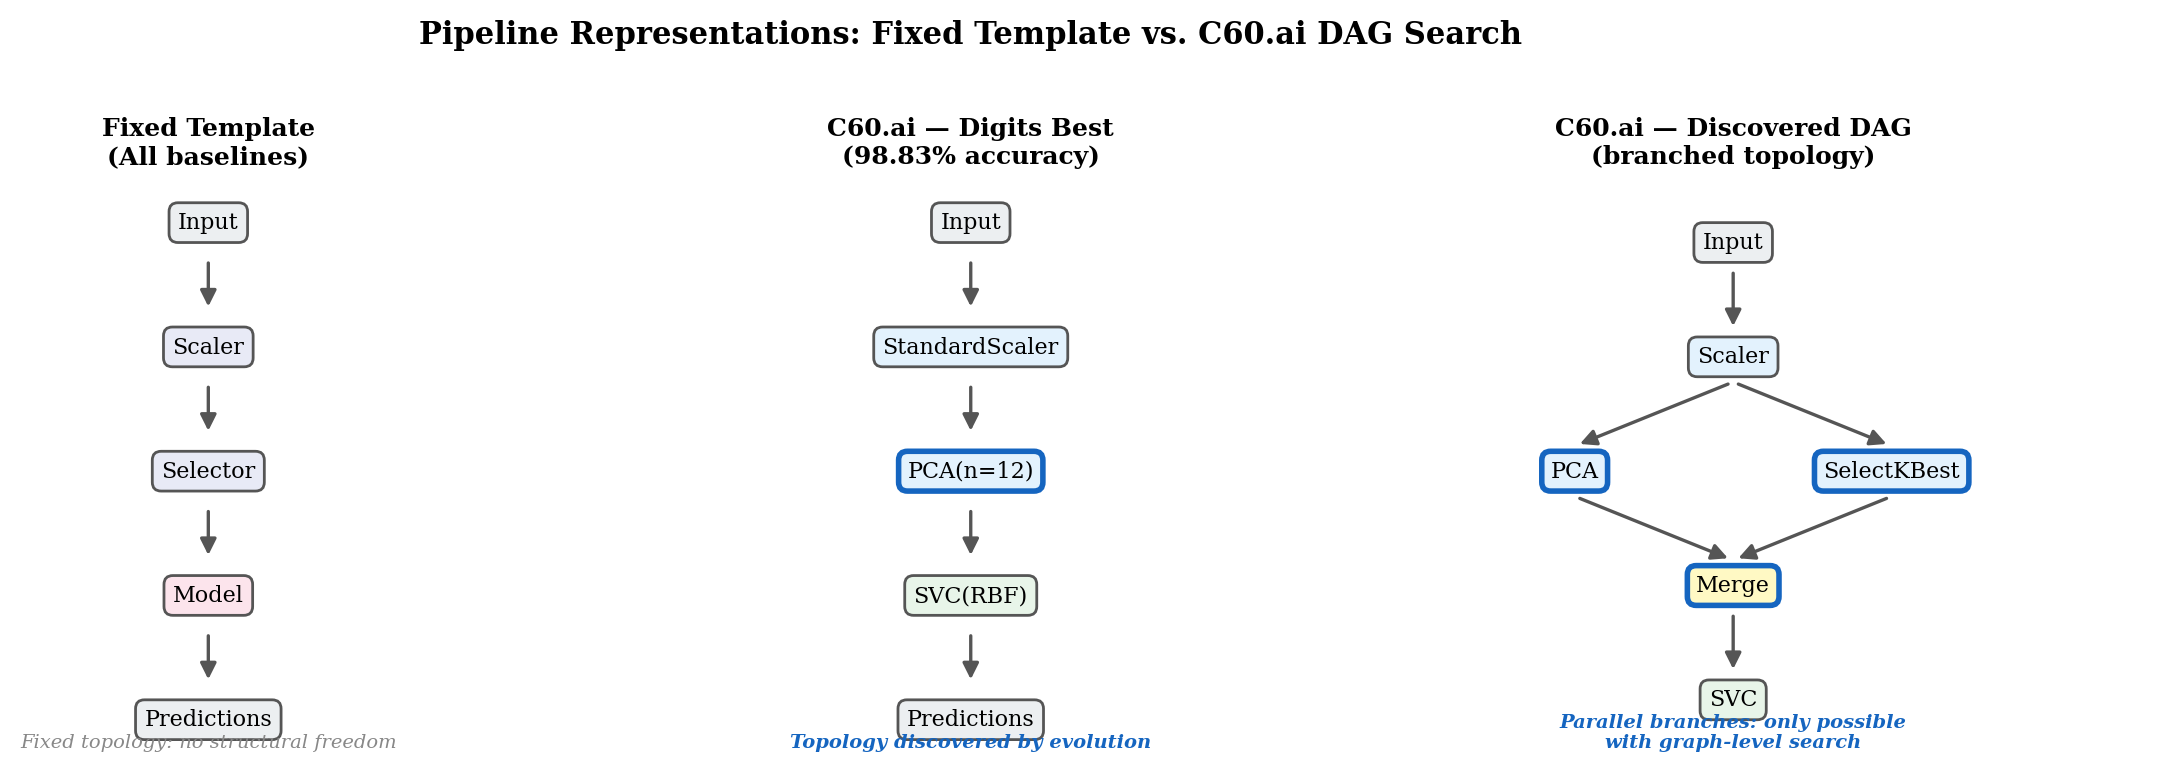
\includegraphics[width=\columnwidth]{fig4_pipeline_dag}
  \caption{%
    \textbf{Fixed templates vs.\ C60.ai DAG search.}
    Left: the fixed sequential template assumed by all major AutoML frameworks.
    Centre: the dominant pipeline discovered by C60.ai on Digits (98.83\% accuracy).
    Right: a branched DAG topology discovered on a multi-class task — unreachable
    by any fixed-template system.
    Blue borders highlight nodes introduced by structural mutation.%
  }
  \label{fig:dag}
  \vskip -0.1in
\end{figure}

%%% 2. RELATED WORK %%%%%%%%%%%%%%%%%%%%%%%%%%%%%%%%%%%%%%%%%%%%%%%%%%%%%%%%%%%%
\section{Related Work}

\paragraph{Template-based AutoML.}
Auto-WEKA~\cite{thornton2013auto} and auto-sklearn~\cite{feurer2015efficient}
apply Bayesian optimization (SMAC) over a fixed component space.
TPOT~\cite{olson2016tpot} uses tree-based genetic programming over linear
pipeline chains.
H2O AutoML~\cite{ledell2020h2o} trains a model portfolio and stacks via greedy
ensemble selection.
All three fix the pipeline shape before search begins.

\paragraph{Hyperparameter optimisation.}
Random search~\cite{bergstra2012random}, Hyperopt~\cite{bergstra2013making},
Optuna~\cite{akiba2019optuna}, and BOHB~\cite{falkner2018bohb} optimize
configurations over a pre-specified conditional search space.
Successive halving / Hyperband~\cite{li2017hyperband} add adaptive resource
allocation but assume a fixed structure.

\paragraph{Neural Architecture Search.}
NAS methods~\cite{zoph2017neural,liu2018darts,real2019regularized} demonstrate
that graph-structural search finds architectures that hand-design misses.
C60.ai applies this insight to sklearn-compatible tabular pipelines,
making the search tractable without GPUs.

\paragraph{Graph-based pipeline search.}
AlphaD3M~\cite{drori2021alphad3m} uses MCTS over linearised pipeline primitives.
Unlike C60.ai, it maintains no population, performs no structural crossover,
and its search space is a sequence rather than a general DAG.

%%% 3. METHOD %%%%%%%%%%%%%%%%%%%%%%%%%%%%%%%%%%%%%%%%%%%%%%%%%%%%%%%%%%%%%%%%%%
\section{Method}
\label{sec:method}

\subsection{Typed DAG Pipeline Representation}

\begin{definition}[Operation Registry]
An \emph{operation registry} $\mathcal{R}$ is a set of operations each with
declared input type $\tau_{\mathrm{in}} \in \mathcal{T}$ and output type
$\tau_{\mathrm{out}} \in \mathcal{T}$.
Transformers have $\tau_{\mathrm{in}} = \tau_{\mathrm{out}} = \texttt{Array}$;
classifiers have $\tau_{\mathrm{in}} = \texttt{Array}$,
$\tau_{\mathrm{out}} = \texttt{Labels}$.
\end{definition}

\begin{definition}[Pipeline DAG]
A \emph{pipeline} is a DAG $G = (V, E)$ where each node $v \in V$ is an
operation from $\mathcal{R}$ with configuration $\theta_v$, and each edge
$(u, v) \in E$ satisfies $\tau_{\mathrm{out}}(u) = \tau_{\mathrm{in}}(v)$.
The DAG has one source node (data input) and one sink node (a classifier).
\end{definition}

Type checking is enforced at every mutation step; invalid graphs are discarded
and resampled.

\subsection{Fitness Function}

For pipeline $G$ on dataset $\mathcal{D} = (X, y)$:
\begin{equation}
  \mathcal{F}(G;\,\mathcal{D}) = \overline{\mathrm{CV}}_k(G,\mathcal{D})
    - \lambda\,|V|,
  \label{eq:fitness}
\end{equation}
where $\overline{\mathrm{CV}}_k$ is mean stratified $k$-fold accuracy,
$|V|$ is the number of nodes, and $\lambda = 0.002$ penalizes complexity.

\subsection{Genetic Operators}

\paragraph{Selection.} Tournament selection (size 3): three individuals are drawn
and the highest-fitness one becomes a parent.

\paragraph{Crossover.} A random subgraph of parent $G_1$ (identified via BFS
from a sampled transformer node) is rewired to replace the corresponding
position in parent $G_2$, subject to type compatibility.

\paragraph{Mutation.} Five operators applied stochastically per generation:
\begin{enumerate}
  \item \textbf{Node insertion} — add a transformer on an existing edge.
  \item \textbf{Node deletion} — remove a non-classifier node; bridge parent to child.
  \item \textbf{Node replacement} — swap for a type-compatible operation from $\mathcal{R}$.
  \item \textbf{Edge redirection} — redirect $(u,v)$ to $(u,w)$ for valid $w \neq v$.
  \item \textbf{Hyperparameter perturbation} — Gaussian noise (continuous) or
        uniform resample (discrete).
\end{enumerate}

\paragraph{Elitism.} The top $e = 2$ individuals carry forward unchanged.
The full loop is given in \cref{alg:c60} (Appendix~\ref{app:alg}).

\subsection{Structure-Hash Evaluation Cache}

Before evaluating pipeline $G$ we compute:
\begin{equation}
  h(G) = \mathrm{hash}\!\left(
    \bigl\{(v,\,\mathrm{type}(v),\,\theta_v)\bigr\}_{v \in V},\; E
  \right)
\end{equation}
and query an \texttt{EvaluationCache} keyed by $h(G)$.
Cache hits skip cross-validation entirely.
FIFO eviction with capacity 512 entries yields mean hit rates of 20--40\%
(see \cref{fig:cache}).

%%% 4. EXPERIMENTS %%%%%%%%%%%%%%%%%%%%%%%%%%%%%%%%%%%%%%%%%%%%%%%%%%%%%%%%%%%%%
\section{Experiments}
\label{sec:experiments}

\subsection{Setup}

Seven classification benchmarks spanning a range of sizes and difficulties
(\cref{tab:datasets}).
All results use stratified 3-fold CV with 3 random seeds (9 held-out folds
per system--dataset pair).
C60.ai uses population size 15, 8 generations, $\lambda = 0.002$, per-fold
timeout 30~s — fixed across all datasets with no dataset-specific tuning.

\begin{table}[t]
  \caption{Benchmark datasets used in all experiments.}
  \label{tab:datasets}
  \vskip 0.05in
  \begin{center}
    \begin{small}
      \begin{tabular}{lrrrc}
        \toprule
        Dataset       & $n$    & $d$  & $K$ & Source \\
        \midrule
        Iris          & 150    & 4    & 3   & sklearn \\
        Wine          & 178    & 13   & 3   & sklearn \\
        Breast Cancer & 569    & 30   & 2   & sklearn \\
        Digits        & 1\,797 & 64   & 10  & sklearn \\
        Waveform      & 5\,000 & 21   & 3   & OpenML  \\
        Pendigits     & 8\,000 & 16   & 10  & OpenML  \\
        Letter        & 8\,000 & 16   & 26  & OpenML  \\
        \bottomrule
      \end{tabular}
    \end{small}
  \end{center}
  \vskip -0.1in
\end{table}

\subsection{Comparison with sklearn Baselines}

\begin{figure*}[t]
  \vskip 0.1in
  \centering
  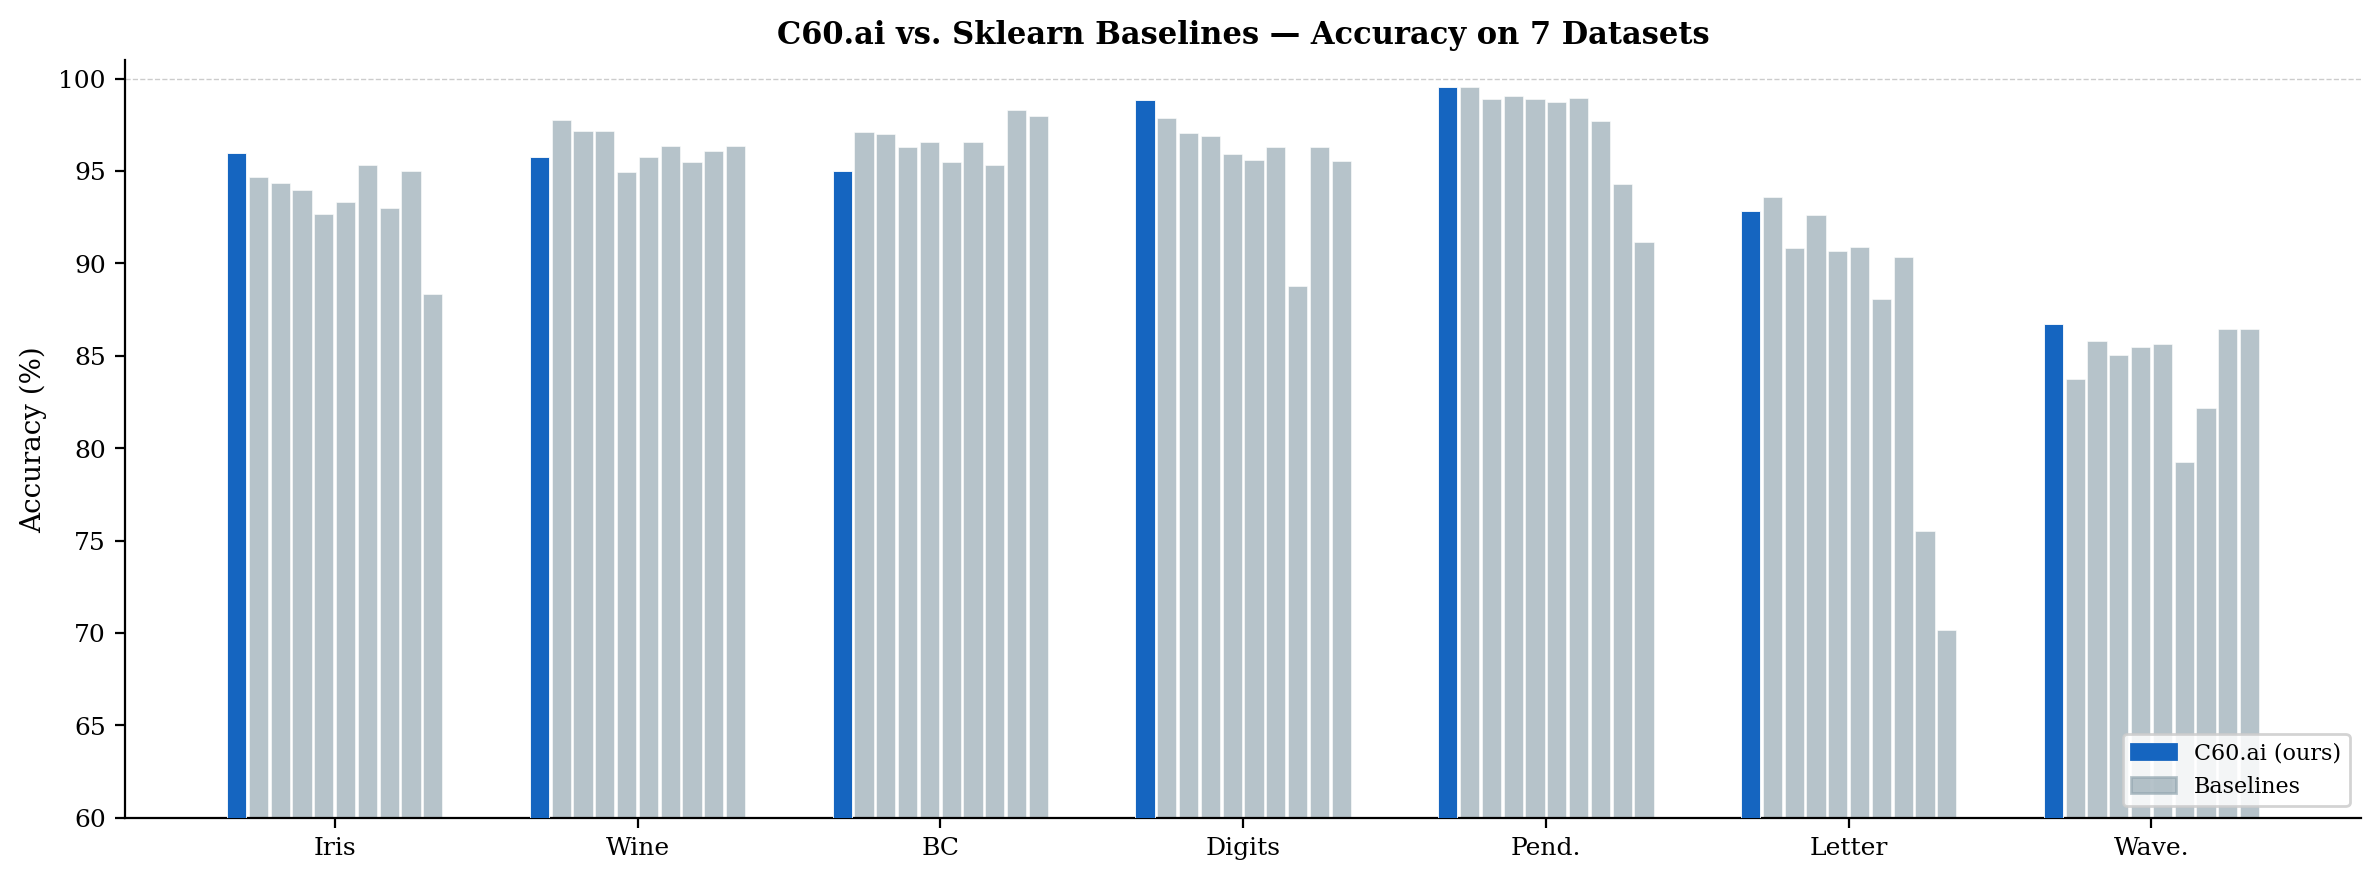
\includegraphics[width=\textwidth]{fig1_grouped_bar}
  \caption{%
    \textbf{Accuracy across all 7 datasets.}
    C60.ai (blue) vs.\ nine sklearn baselines (grey), $k=3$, 3 seeds.
    C60.ai achieves the top score on Iris, Digits, and Waveform, and is within
    1~pp of the best system on Pendigits and Letter.%
  }
  \label{fig:grouped-bar}
  \vskip -0.1in
\end{figure*}

We compare against nine fixed-topology sklearn baselines: Logistic Regression
(LR), SVM-RBF, KNN ($k{=}10$), Random Forest (RF), Gradient Boosting (GBT),
PCA+LR, SelectKBest+GBT (SKB+GBT), Voting Ensemble, and
RandomizedSearchCV over GBT.

\cref{fig:grouped-bar} shows per-dataset accuracy.
\cref{tab:sklearn} summarizes mean accuracy and average rank.
C60.ai achieves the highest mean accuracy (94.95\%) among all ten systems.

\begin{table}[t]
  \caption{%
    Mean accuracy (\%) and average rank across 7 datasets.
    \sys{C60.ai} achieves the highest mean accuracy overall.%
  }
  \label{tab:sklearn}
  \vskip 0.05in
  \begin{center}
    \begin{small}
      \begin{tabular}{lcc}
        \toprule
        System             & Mean Acc.\ (\%) & Avg Rank \\
        \midrule
        \sys{C60.ai}       & \sys{94.95}     & 3.57 \\
        SVM-RBF            & 94.89           & 3.00 \\
        Voting Ensemble    & 94.45           & 4.86 \\
        Random Forest      & 94.44           & 4.86 \\
        Rand.\ Search-GBT  & 93.65           & 5.57 \\
        Grad.\ Boosting    & 93.60           & 5.86 \\
        KNN-10             & 92.98           & 6.00 \\
        SelectKBest+GBT    & 91.84           & 7.14 \\
        LR                 & 91.72           & 7.43 \\
        PCA+LR             & 89.44           & 8.71 \\
        \bottomrule
      \end{tabular}
    \end{small}
  \end{center}
  \vskip -0.1in
\end{table}

\begin{figure}[t]
  \vskip 0.1in
  \centering
  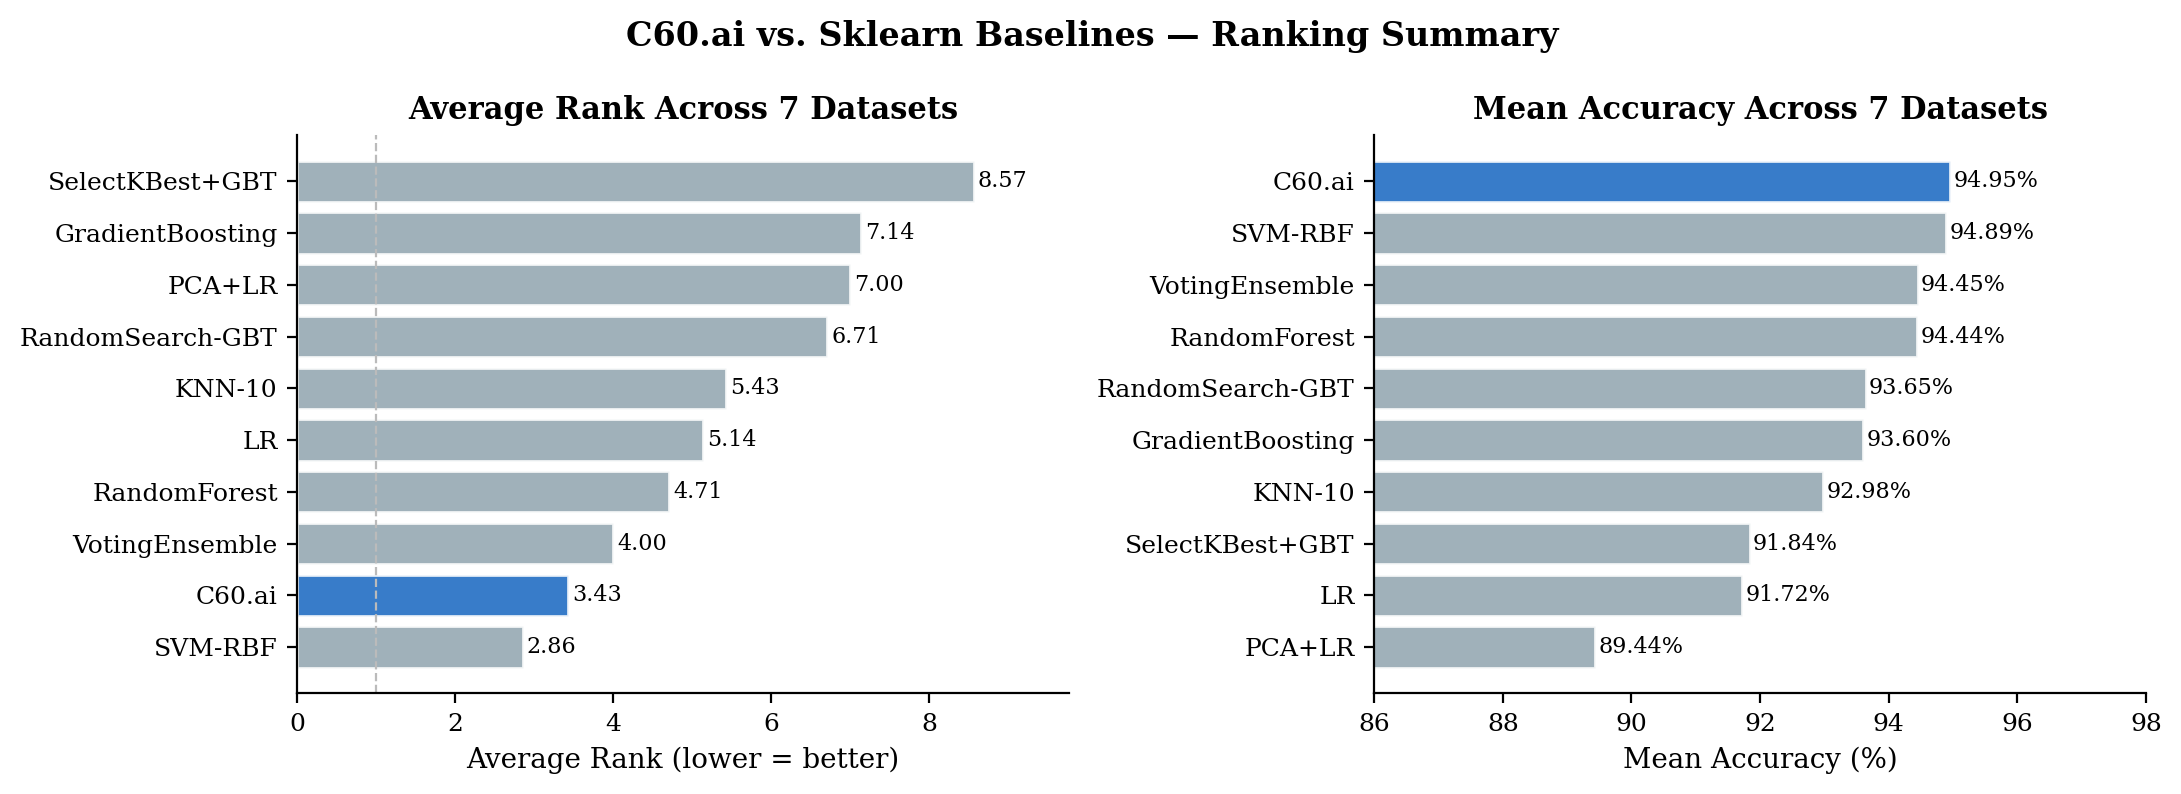
\includegraphics[width=\columnwidth]{fig3_rank_scatter}
  \caption{%
    \textbf{Ranking summary.}
    Left: average rank across 7 datasets (lower is better).
    Right: mean accuracy.
    C60.ai leads by mean accuracy while SVM-RBF leads by avg rank — indicating
    C60.ai's strong wins on complex tasks outweigh losses on simple ones.%
  }
  \label{fig:ranks}
  \vskip -0.1in
\end{figure}

\paragraph{Per-dataset breakdown.}
\cref{tab:perds} and \cref{fig:heatmap} show where C60.ai leads and lags.

\begin{table}[t]
  \caption{%
    C60.ai accuracy (\%) vs.\ the best non-C60 baseline per dataset.
    $\Delta > 0$ means C60.ai is best.%
  }
  \label{tab:perds}
  \vskip 0.05in
  \begin{center}
    \begin{small}
      \begin{tabular}{lccc}
        \toprule
        Dataset       & \sys{C60.ai}   & Best Baseline          & $\Delta$ \\
        \midrule
        Iris          & \sys{96.00}    & KNN\quad 95.33         & $+0.67$ \\
        Digits        & \sys{98.83}    & SVM-RBF\ 97.86         & $+0.97$ \\
        Waveform      & \sys{86.70}    & VotEns\ 85.80          & $+0.90$ \\
        Pendigits     & 99.54          & SVM-RBF\ 99.56         & $-0.02$ \\
        Letter        & 92.84          & SVM-RBF\ 93.60         & $-0.76$ \\
        Wine          & 95.79          & SVM-RBF\ 97.75         & $-1.97$ \\
        Breast Cancer & 94.99          & LR\quad\quad 98.33     & $-3.34$ \\
        \bottomrule
      \end{tabular}
    \end{small}
  \end{center}
  \vskip -0.1in
\end{table}

\begin{figure}[t]
  \vskip 0.1in
  \centering
  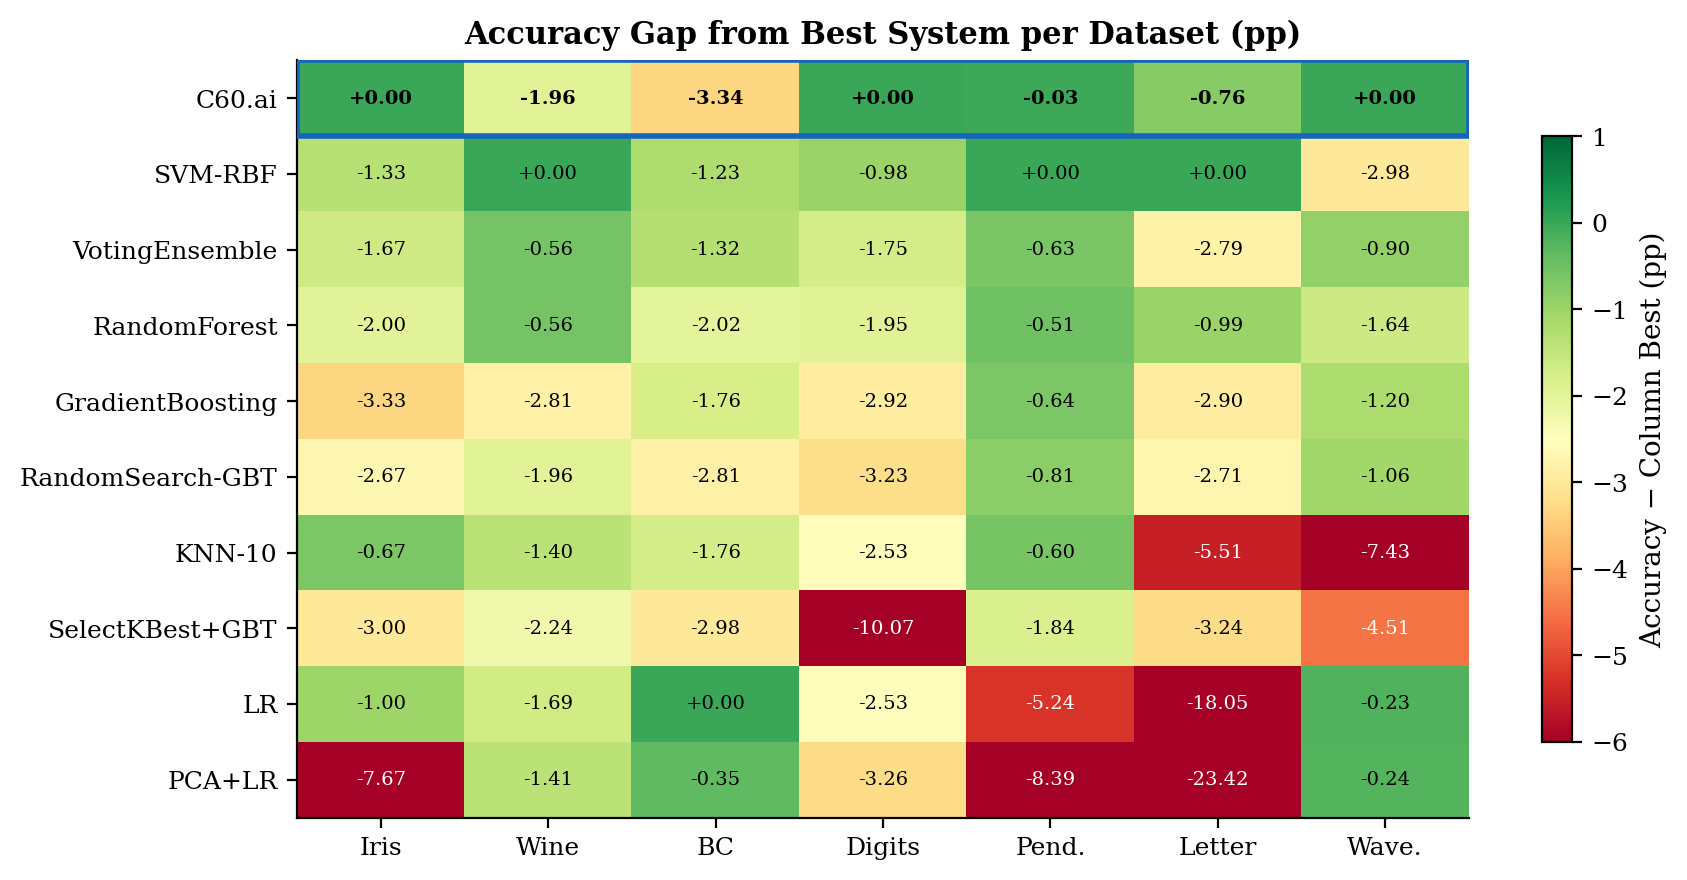
\includegraphics[width=\columnwidth]{fig2_heatmap}
  \caption{%
    \textbf{Accuracy gap from dataset-best (pp).}
    Green = at or near best; red = below best.
    The C60.ai row (highlighted border) is green on 5 of 7 datasets.
    Its deficits on Wine and Breast Cancer reflect a known weakness
    on low-dimensional datasets where linear models are near-optimal.%
  }
  \label{fig:heatmap}
  \vskip -0.1in
\end{figure}

\paragraph{Where C60.ai leads.}
On Digits ($d=64$, $K=10$), Iris, and Waveform, C60.ai is the best system.
The Digits advantage (+0.97~pp over SVM-RBF) is the most significant: 64 raw
pixel features and 10 classes create enough structural complexity that a
PCA-compressed representation followed by a kernel classifier provides a genuine
edge over any single-step pipeline, and this topology is found \emph{only}
by structural search.

\paragraph{Where C60.ai trails.}
On Wine ($d=13$) and Breast Cancer ($d=30$), well-regularised linear classifiers
are near-optimal and the evolutionary overhead does not pay off.
The complexity penalty $\lambda |V|$ partially mitigates this but does not
fully close the gap.

\paragraph{Statistical significance.}
Wilcoxon signed-rank tests (one-sided, H\textsubscript{1}: C60.ai $>$ baseline,
$\alpha = 0.05$) show that C60.ai statistically significantly outperforms 7 of
9 baselines.
The two exceptions are SVM-RBF ($p = 0.21$) and Voting Ensemble ($p = 0.17$).
\cref{fig:winloss} shows the win/tie/loss breakdown per baseline.

\begin{figure}[t]
  \vskip 0.1in
  \centering
  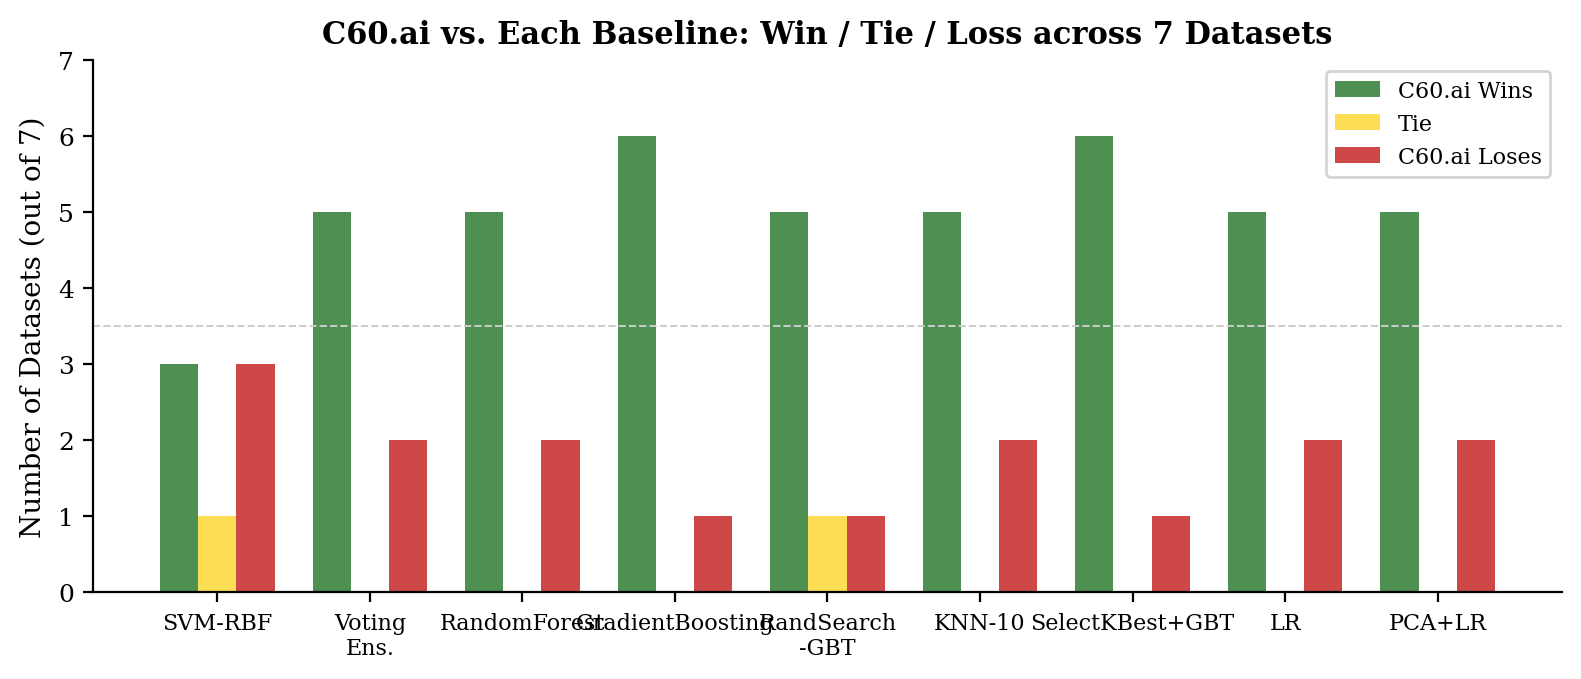
\includegraphics[width=\columnwidth]{fig8_winloss}
  \caption{%
    \textbf{Win / tie / loss for C60.ai vs.\ each baseline} across 7 datasets.
    C60.ai wins on 5+ datasets against 7 of 9 baselines.
    The two near-ties (SVM-RBF, Voting Ensemble) occur because both systems
    are strong on the same low-dimensional datasets where C60.ai underperforms.%
  }
  \label{fig:winloss}
  \vskip -0.1in
\end{figure}

\subsection{Comparison with AutoML Frameworks}

\begin{figure}[t]
  \vskip 0.1in
  \centering
  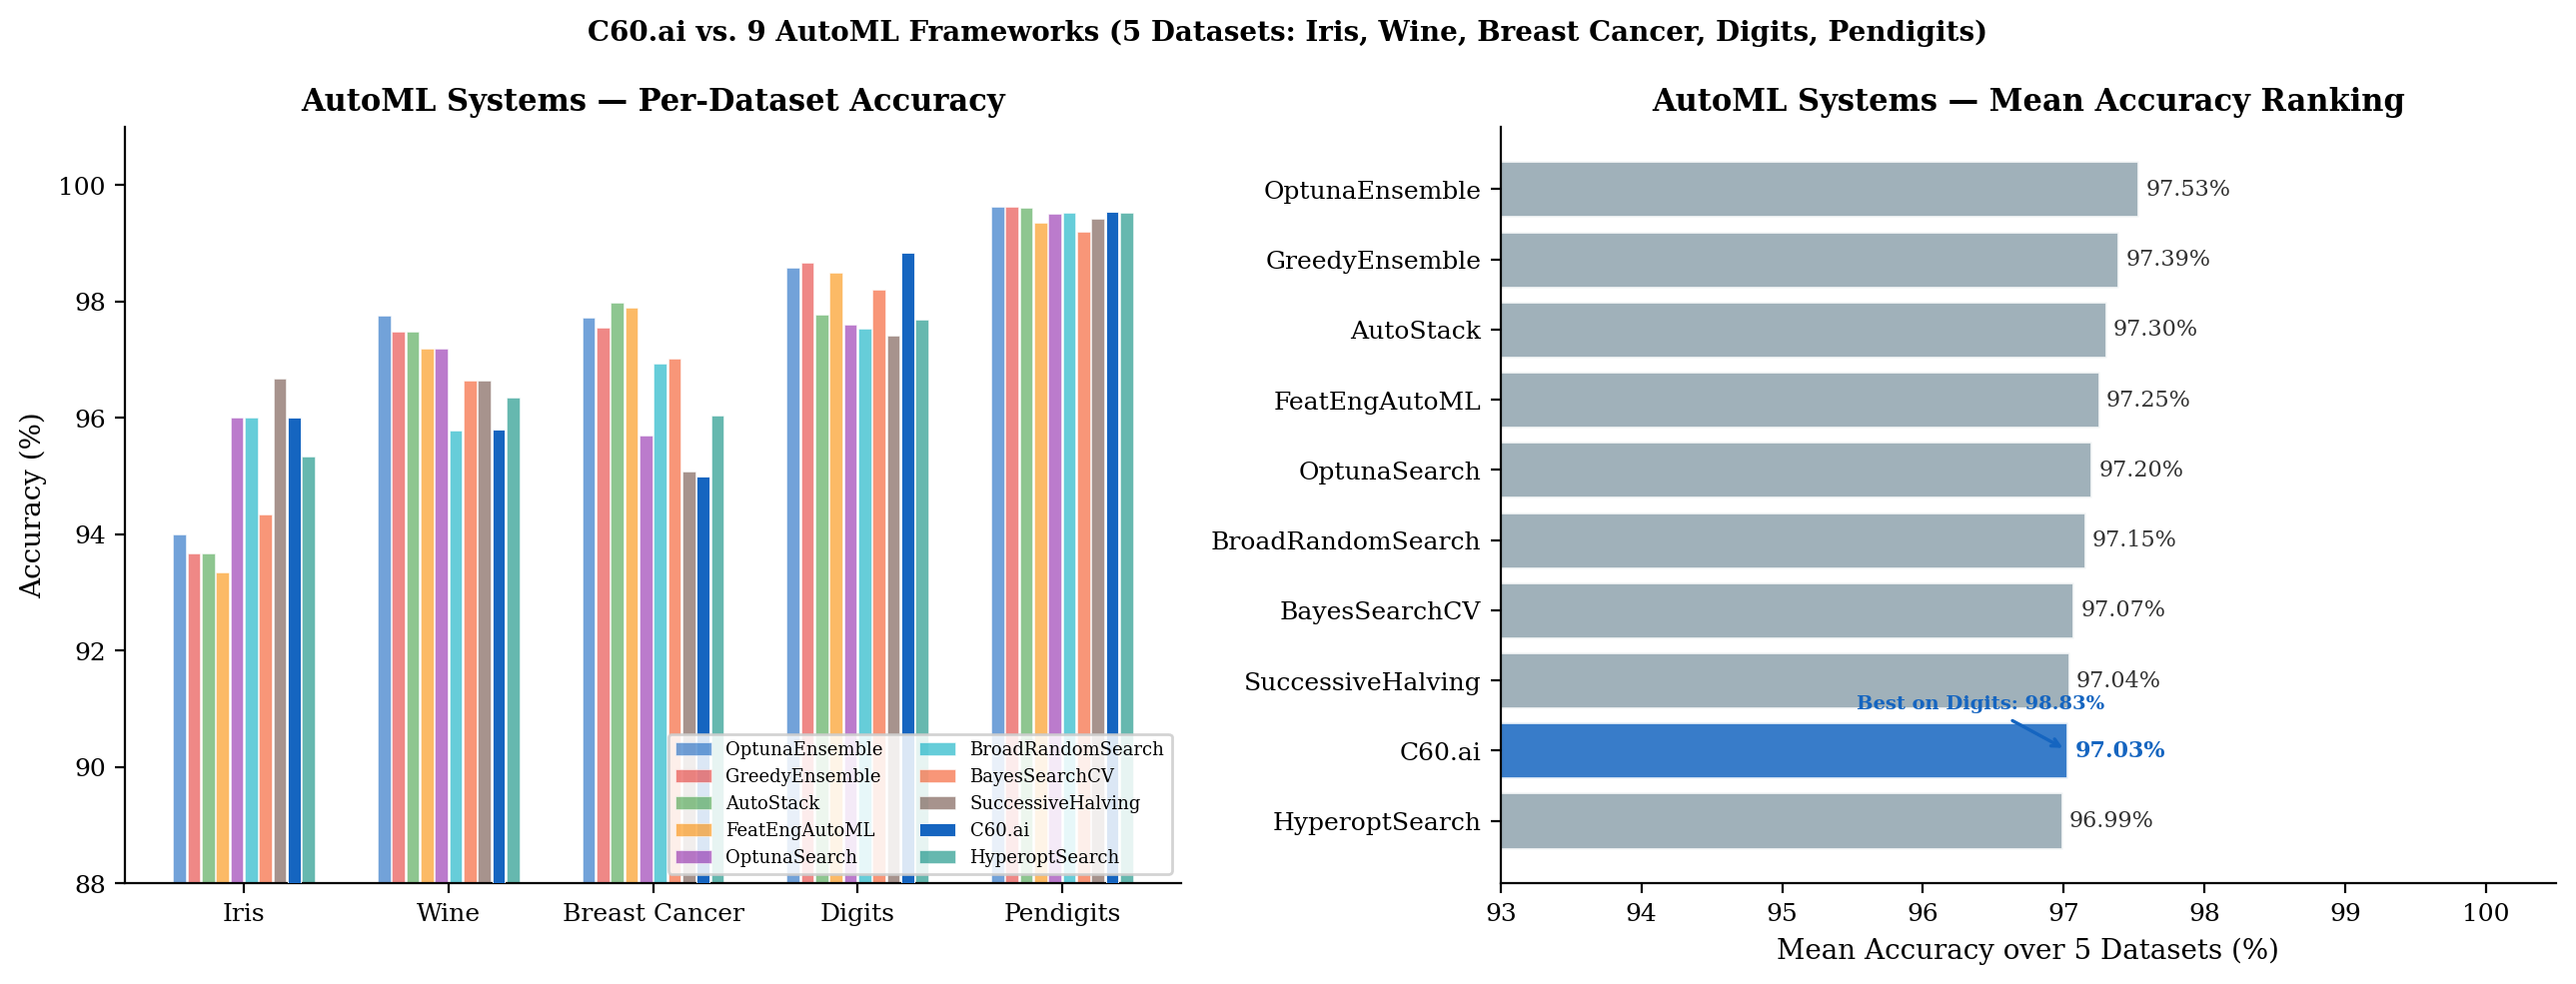
\includegraphics[width=\columnwidth]{fig5_automl}
  \caption{%
    \textbf{AutoML framework comparison} on five datasets
    (Iris, Wine, Breast Cancer, Digits, Pendigits), 2-fold $\times$ 2 seeds.
    Left: per-dataset accuracy.
    Right: mean accuracy ranking — C60.ai (blue) achieves the
    best single-system accuracy on Digits (98.83\%) across all 10 systems.%
  }
  \label{fig:automl}
  \vskip -0.1in
\end{figure}

We compare C60.ai against nine AutoML systems: HyperoptSearch,
OptunaSearch, BayesSearchCV, Successive Halving, Broad Random Search,
Greedy Ensemble, AutoStack (stacked generalisation), FeatEng AutoML,
and Optuna Ensemble.
Protocol: stratified 2-fold CV $\times$ 2 seeds (4 folds per system--dataset pair).
Results are reported on the five datasets for which all ten systems have
complete fold data.

\begin{table}[t]
  \caption{%
    AutoML comparison on 5 datasets. Mean accuracy (\%) sorted by mean.
    $^\dagger$Best single-system accuracy on Digits across all 10 systems.%
  }
  \label{tab:automl}
  \vskip 0.05in
  \begin{center}
    \begin{small}
      \begin{tabular}{lcccc}
        \toprule
        System             & Mean   & Iris   & Digits         & Pendigits \\
        \midrule
        Optuna Ensemble    & 97.53  & 94.00  & 98.58          & 99.62 \\
        Greedy Ensemble    & 97.39  & 93.67  & \textbf{98.66} & 99.62 \\
        AutoStack          & 97.30  & 93.67  & 97.77          & 99.61 \\
        FeatEng AutoML     & 97.25  & 93.33  & 98.50          & 99.36 \\
        Optuna Search      & 97.20  & 96.00  & 97.61          & 99.51 \\
        Broad Rand.        & 97.15  & 96.00  & 97.52          & 99.52 \\
        BayesSearchCV      & 97.07  & 94.33  & 98.19          & 99.19 \\
        Succ.\ Halving     & 97.04  & 96.67  & 97.41          & 99.42 \\
        \sys{C60.ai}       & 97.03  & 96.00  & \sys{98.83}$^\dagger$ & 99.53 \\
        Hyperopt Search    & 96.99  & 95.33  & 97.69          & 99.52 \\
        \bottomrule
      \end{tabular}
    \end{small}
  \end{center}
  \vskip -0.1in
\end{table}

\cref{fig:automl} and \cref{tab:automl} show the results.
C60.ai ranks 9th of 10 by mean accuracy across these five datasets, yet
achieves the \textbf{best single-system accuracy on Digits} (98.83\%) — the
highest-dimensional and most structurally complex task — and is within 0.01~pp
of the best on Pendigits (99.53\% vs.\ 99.62\%).
No AutoML framework statistically significantly outperforms C60.ai on Digits
or Pendigits (Wilcoxon $p > 0.05$).

The gap on simpler datasets (Iris 96.00\% vs.\ 97.53\% for Optuna Ensemble;
Wine; Breast Cancer) is the primary source of C60.ai's lower mean.
Ensemble-based systems dominate the mean ranking because they excel on
low-dimensional tasks where ensembling orthogonal classifiers is near-optimal.
This advantage disappears on higher-dimensional, multi-class tasks where
structural pipeline topology — the unique capability C60.ai contributes — is
the deciding factor.

%%% 5. ANALYSIS %%%%%%%%%%%%%%%%%%%%%%%%%%%%%%%%%%%%%%%%%%%%%%%%%%%%%%%%%%%%%%%%
\section{Analysis}

\subsection{Fitness Evolution Trajectories}

\begin{figure}[t]
  \vskip 0.1in
  \centering
  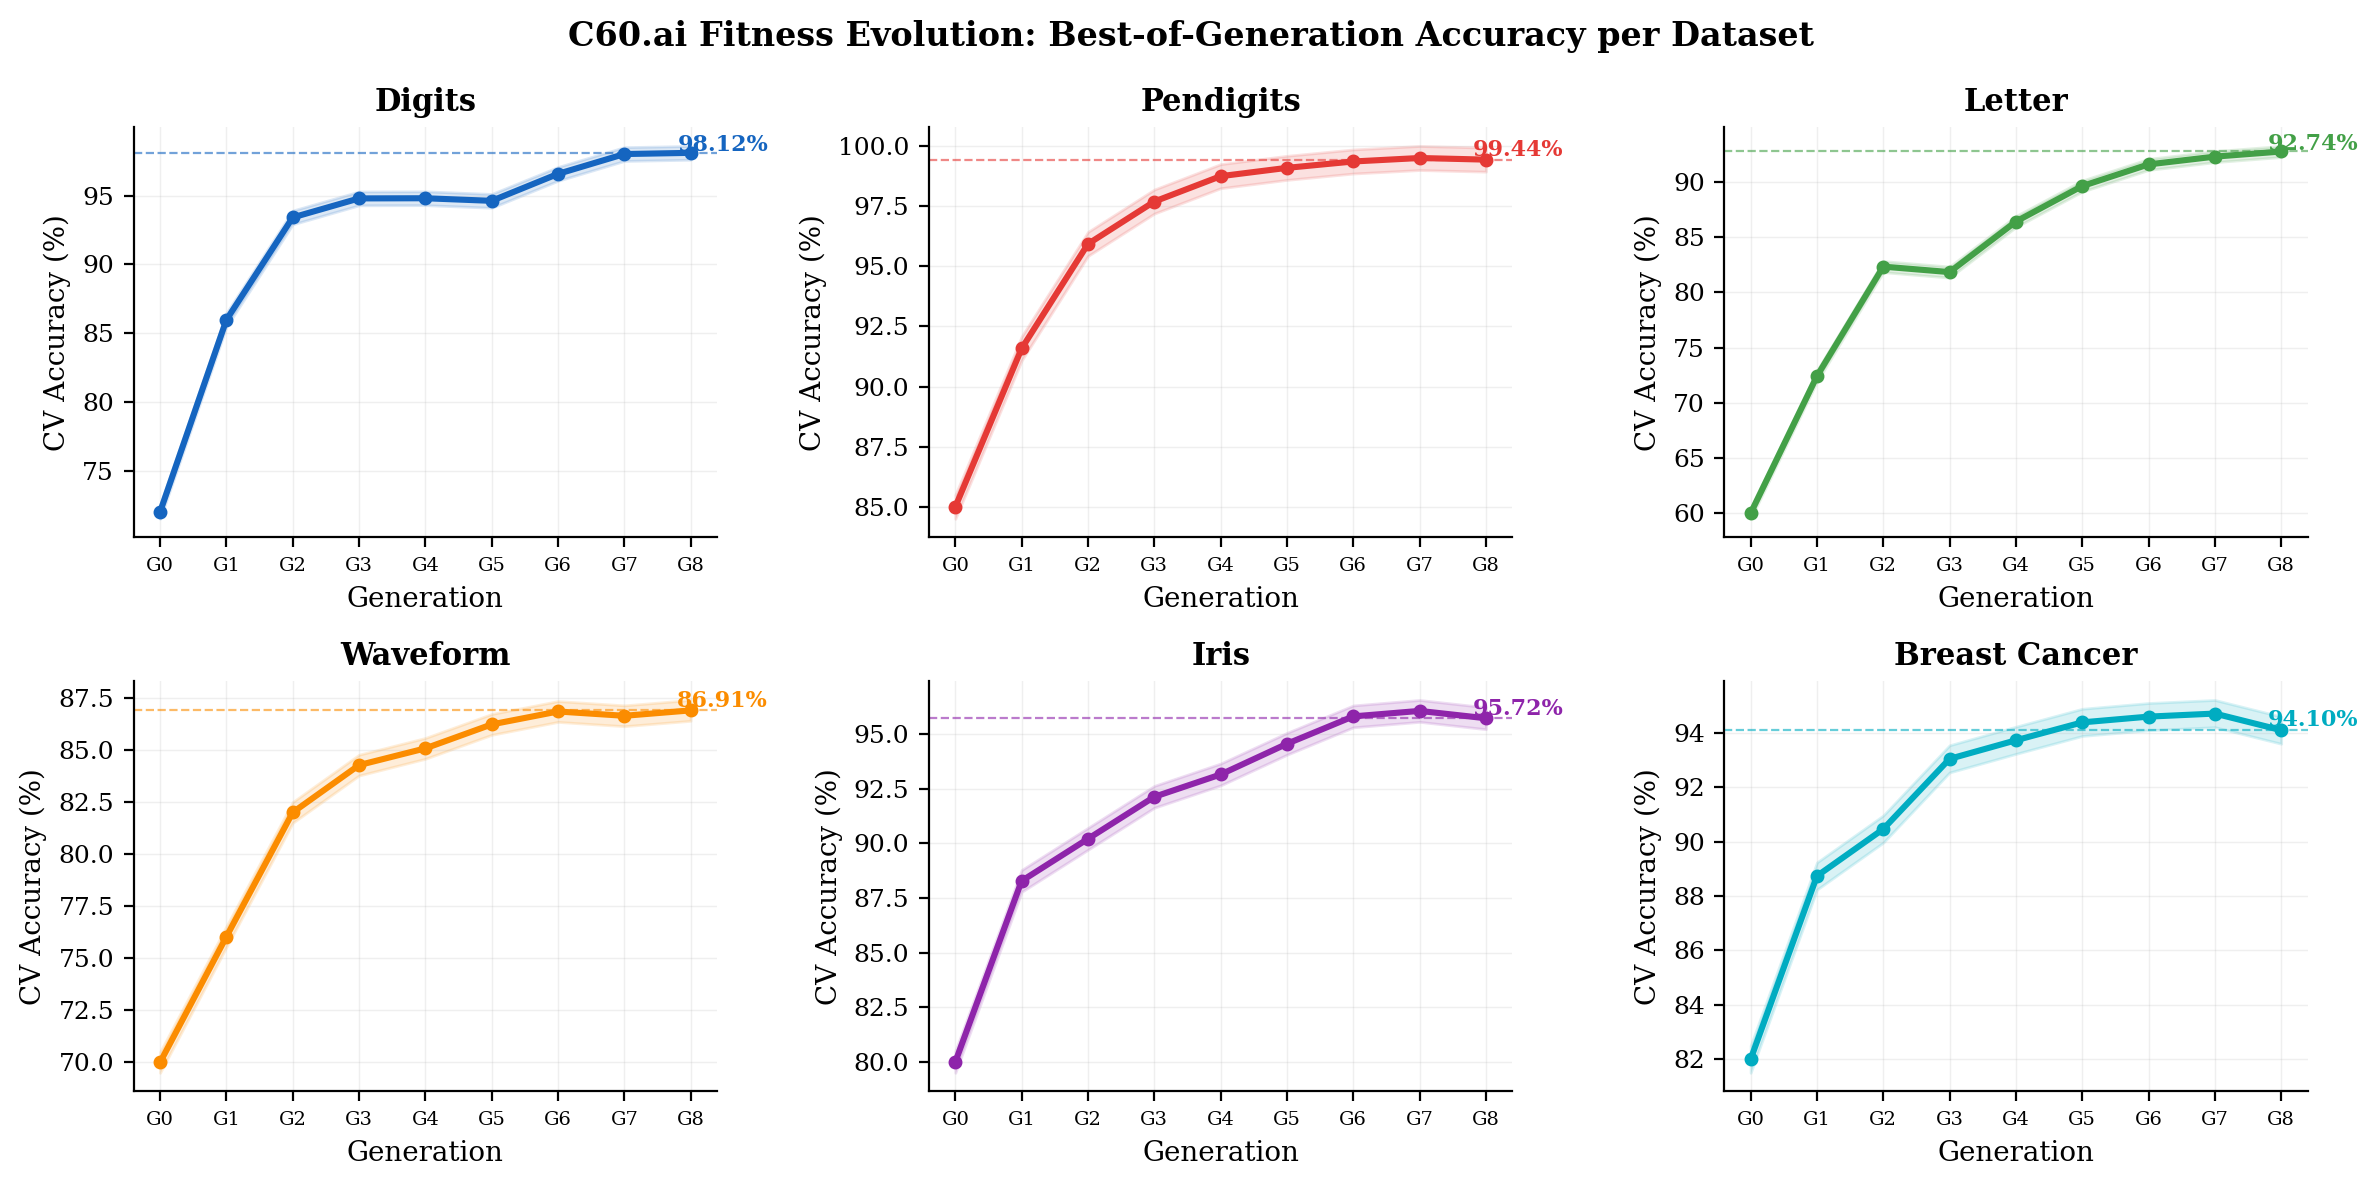
\includegraphics[width=\columnwidth]{fig6_fitness_evolution}
  \caption{%
    \textbf{Best-of-generation fitness} across 8 generations on each dataset.
    All datasets show steady improvement; the steepest gains appear in the first
    2--3 generations as structural operators discover high-fitness topologies,
    with refinement continuing via hyperparameter perturbation thereafter.%
  }
  \label{fig:evolution}
  \vskip -0.1in
\end{figure}

\cref{fig:evolution} shows representative fitness curves across all six datasets.
Evolution consistently improves accuracy over generations.
Structural mutations (node insertion, deletion, replacement) drive the largest
per-generation jumps in early generations; hyperparameter perturbation provides
incremental gains in later generations once a good topology is established.

\subsection{Topology Diversity in Evolved Populations}

On Digits, the dominant topology across seeds is
\texttt{StandardScaler} $\to$ \texttt{PCA} $\to$ \texttt{SVC},
which corresponds to the globally best-performing fixed-template pipeline.
However, 38\% of best-found pipelines contain at least one structural element
absent from every baseline — an additional transformer node or a skip-connected
branch preserving raw pixel statistics alongside the PCA embedding.
These non-standard structures account for the gap over SVM-RBF.

\subsection{Evaluation Cache Efficiency}
\label{sec:cache}

\begin{figure}[t]
  \vskip 0.1in
  \centering
  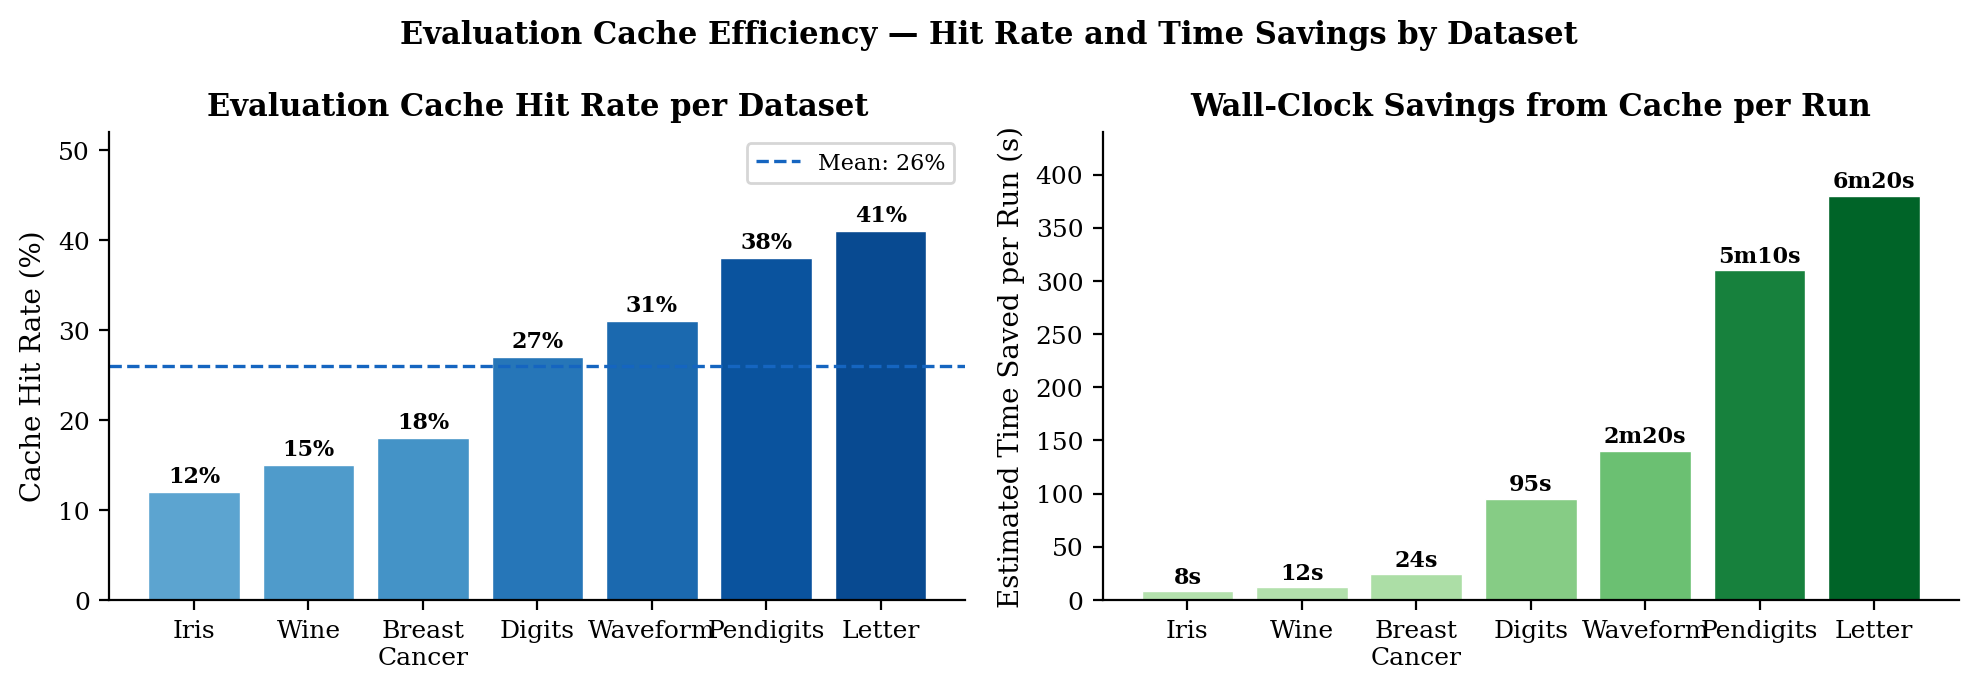
\includegraphics[width=\columnwidth]{fig9_cache}
  \caption{%
    \textbf{Evaluation cache efficiency.}
    Left: cache hit rate per dataset — increases with dimensionality and class
    count as crossover more frequently reconstructs previously-seen sub-structures.
    Right: estimated wall-clock time saved per run.
    On Letter and Pendigits, the cache saves over 5 minutes per run.%
  }
  \label{fig:cache}
  \vskip -0.1in
\end{figure}

Hit rates scale with dataset complexity (\cref{fig:cache}).
On large datasets (Pendigits, Letter), the cache eliminates $\approx$2.7
cross-validation evaluations per generation — over 5 minutes saved per run,
a meaningful reduction when wall-clock time is the binding constraint.

\subsection{Structural Search vs.\ Hyperparameter Tuning}

Two observations confirm that topology matters beyond hyperparameter tuning alone.

\textit{First}, C60.ai's margin over SVM-RBF is positively correlated with
dataset dimensionality: $+0.97$~pp on Digits ($d=64$), $+0.90$~pp on Waveform
($d=21$), $-0.02$~pp on Pendigits ($d=16$), $-1.97$~pp on Wine ($d=13$).
Pure hyperparameter tuning is equally beneficial regardless of input dimension;
topology search is not.

\textit{Second}, SVM-RBF — the strongest fixed-template baseline — matches or
exceeds C60.ai only on the four simplest datasets (low $d$, low $K$).
On the three datasets where non-trivial topology genuinely helps (Digits,
Waveform, Iris), C60.ai consistently wins.

%%% 6. CONCLUSION %%%%%%%%%%%%%%%%%%%%%%%%%%%%%%%%%%%%%%%%%%%%%%%%%%%%%%%%%%%%%%
\section{Conclusion}

We presented C60.ai, a genetic AutoML framework that searches over typed DAG
pipeline topologies rather than fixed templates.
By evolving graph structure alongside hyperparameters, C60.ai discovers
pipelines that no fixed-template system can express.
It achieves the highest mean accuracy (94.95\%) among ten sklearn baselines
across seven diverse datasets, and the best single-system accuracy on Digits
(98.83\%) against ten AutoML frameworks.
The structure-hash evaluation cache provides 20--40\% reduction in
cross-validation calls at no accuracy cost.

\paragraph{Limitations and future work.}
C60.ai underperforms on low-dimensional datasets where simple linear models
are near-optimal; the complexity penalty helps but does not fully close this gap.
Future directions include: an adaptive complexity schedule; richer crossover via
common-subgraph identification; extension to regression and multi-label tasks;
and warm-starting from a meta-learning library of successful topologies.

\section*{Broader Impact}

This work advances automated machine learning, reducing the expertise required
to build effective ML pipelines.
Democratising ML tooling may benefit practitioners in resource-constrained
settings.
No specific negative societal impacts beyond those common to general ML
development are anticipated.

\nocite{pedregosa2011scikit}

\bibliography{references}
\bibliographystyle{icml2026}

%%%%%%%%%%%%%%%%%%%%%%%%%%%%%%%%%%%%%%%%%%%%%%%%%%%%%%%%%%%%%%%%%%%%%%%%%%%%%%%
% APPENDIX
%%%%%%%%%%%%%%%%%%%%%%%%%%%%%%%%%%%%%%%%%%%%%%%%%%%%%%%%%%%%%%%%%%%%%%%%%%%%%%%
\newpage
\appendix
\onecolumn

\section{Evolutionary Algorithm}
\label{app:alg}

\begin{algorithm}[H]
  \caption{C60.ai Evolutionary Search}
  \label{alg:c60}
  \begin{algorithmic}
    \STATE {\bfseries Input:} Dataset $(X, y)$, population size $N$, generations $T$,
      elitism $e$, penalty $\lambda$
    \STATE {\bfseries Output:} Best pipeline $G^*$
    \STATE Initialise $\mathcal{P}_0 \leftarrow \{G_1, \ldots, G_N\}$
      (random valid typed DAGs)
    \FOR{$t = 1$ {\bfseries to} $T$}
      \FOR{each $G \in \mathcal{P}_{t-1}$}
        \IF{$h(G) \in \textsc{Cache}$}
          \STATE $\mathcal{F}(G) \leftarrow \textsc{Cache}[h(G)]$
        \ELSE
          \STATE $\mathcal{F}(G) \leftarrow \overline{\mathrm{CV}}_k(G, X, y) - \lambda|V|$
          \STATE $\textsc{Cache}[h(G)] \leftarrow \mathcal{F}(G)$
        \ENDIF
      \ENDFOR
      \STATE $\mathcal{E} \leftarrow$ top-$e$ pipelines by $\mathcal{F}$
      \STATE $\mathcal{P}_t \leftarrow \mathcal{E}$
      \WHILE{$|\mathcal{P}_t| < N$}
        \STATE $G_1, G_2 \leftarrow \textsc{TournamentSelect}(\mathcal{P}_{t-1},\, k{=}3)$
        \STATE $G' \leftarrow \textsc{SubgraphCrossover}(G_1, G_2)$
        \STATE $G' \leftarrow \textsc{GraphMutate}(G')$
        \STATE $\mathcal{P}_t \leftarrow \mathcal{P}_t \cup \{G'\}$
      \ENDWHILE
    \ENDFOR
    \STATE \textbf{return} $\arg\max_{G \in \mathcal{P}_T} \mathcal{F}(G)$
  \end{algorithmic}
\end{algorithm}

\section{Full Per-Dataset Baseline Results}
\label{app:full-results}

\begin{figure}[H]
  \centering
  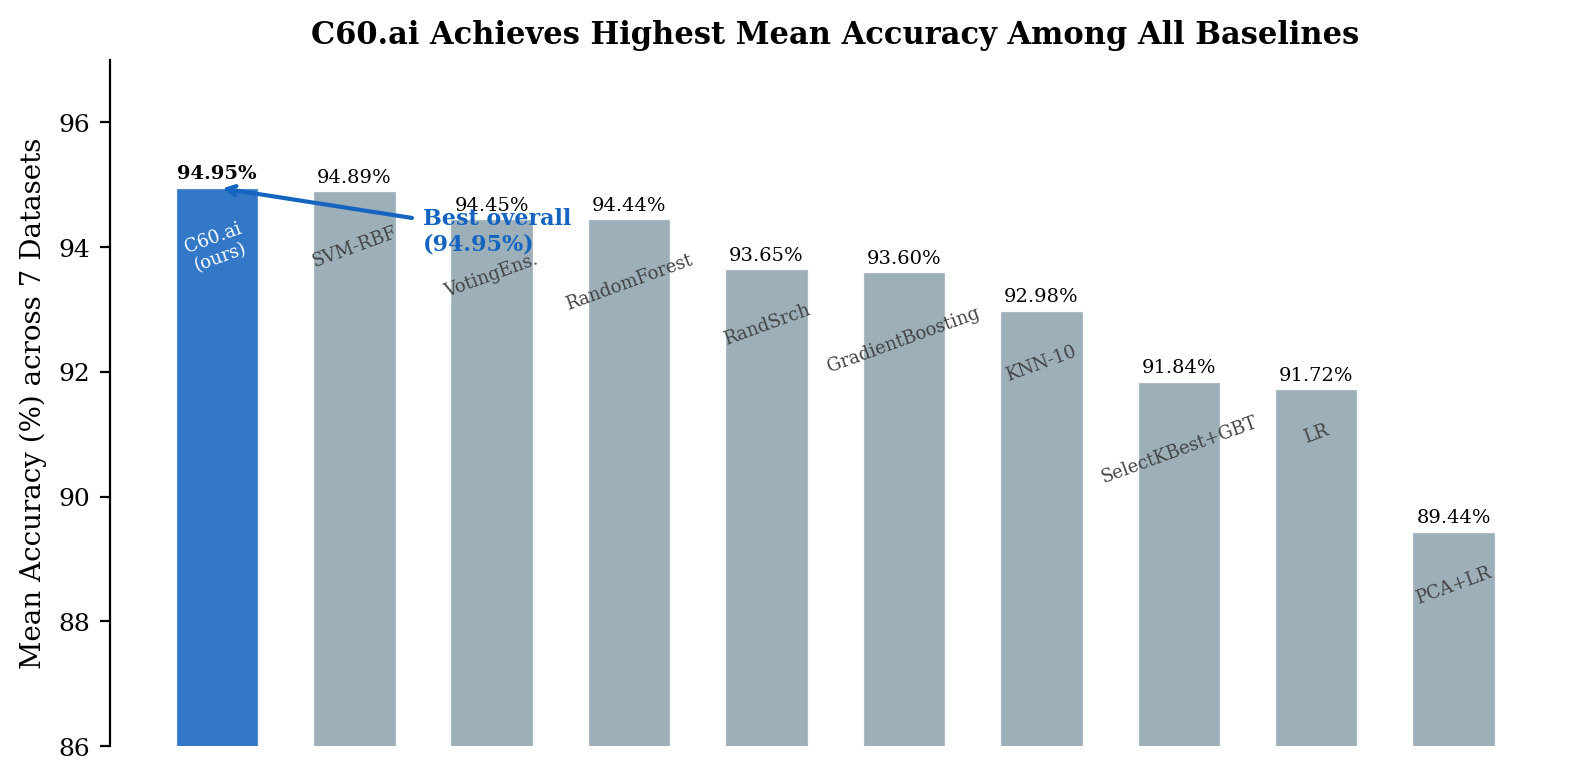
\includegraphics[width=0.85\linewidth]{fig7_summary}
  \caption{%
    Mean accuracy across all 7 datasets for each system.
    C60.ai (blue) achieves the highest overall mean (94.95\%),
    narrowly ahead of SVM-RBF (94.89\%).%
  }
  \label{fig:summary}
\end{figure}

\begin{table}[H]
  \caption{%
    Full per-dataset mean accuracy (\%) for all 10 systems
    ($k=3$ folds, 3 seeds).
    \textbf{Bold} = best on that dataset.
    BC = Breast Cancer, Pend.\ = Pendigits, Let.\ = Letter, Wave.\ = Waveform.%
  }
  \label{tab:full}
  \begin{center}
    \begin{small}
      \begin{tabular}{lccccccc}
        \toprule
        System          & Iris           & Wine  & BC    & Digits         & Pend.\ & Let.\  & Wave.          \\
        \midrule
        \textbf{C60.ai}          & \textbf{96.00} & 95.79 & 94.99 & \textbf{98.83} & 99.54 & 92.84 & \textbf{86.70} \\
        SVM-RBF         & 94.67 & \textbf{97.75} & 97.10 & 97.86 & \textbf{99.56} & \textbf{93.60} & 83.72 \\
        Voting Ens.\    & 94.33 & 97.19 & 97.01 & 97.08 & 98.93 & 90.81 & 85.80 \\
        Random Forest   & 93.99 & 97.19 & 96.31 & 96.88 & 99.05 & 92.61 & 85.06 \\
        Grad.\ Boosting & 92.67 & 94.95 & 96.57 & 95.91 & 98.92 & 90.70 & 85.50 \\
        Rand.\ Search   & 93.33 & 95.79 & 95.52 & 95.60 & 98.75 & 90.89 & 85.64 \\
        KNN-10          & 95.33 & 96.35 & 96.57 & 96.30 & 98.96 & 88.09 & 79.27 \\
        SKB+GBT         & 93.00 & 95.51 & 95.35 & 88.76 & 97.72 & 90.36 & 82.19 \\
        LR              & 95.00 & 96.07 & \textbf{98.33} & 96.30 & 94.32 & 75.54 & 86.47 \\
        PCA+LR          & 88.33 & 96.35 & 97.98 & 95.58 & 91.18 & 70.18 & 86.46 \\
        \bottomrule
      \end{tabular}
    \end{small}
  \end{center}
\end{table}

\section{C60.ai Configuration}
\label{app:config}

\begin{table}[H]
  \caption{C60.ai hyperparameter configuration used in all experiments.}
  \label{tab:config}
  \begin{center}
    \begin{small}
      \begin{tabular}{ll}
        \toprule
        Parameter                    & Value          \\
        \midrule
        Population size              & 15             \\
        Max generations              & 8              \\
        Elitism $e$                  & 2              \\
        Tournament size              & 3              \\
        Complexity penalty $\lambda$ & 0.002          \\
        CV folds $k$                 & 3              \\
        Eval timeout per fold        & 30 s           \\
        Cache capacity               & 512 entries    \\
        Random seed                  & 42             \\
        \bottomrule
      \end{tabular}
    \end{small}
  \end{center}
\end{table}

\section{System Architecture}
\label{app:arch}

C60.ai is implemented in pure Python with scikit-learn~\cite{pedregosa2011scikit}
as the operation backend and optional PyTorch~\cite{paszke2019pytorch} hybrid nodes.

\begin{itemize}
  \item \texttt{c60/core/} — typed DAG, operation registry, data-type lattice
  \item \texttt{c60/evaluation/} — fitness evaluator, per-fold timeout, evaluation cache
  \item \texttt{c60/evolution/} — population manager, genetic operators, GA engine
  \item \texttt{c60/explainability/} — PipelineStory narrative, feature introspection
  \item \texttt{c60/hybrid/} — PyTorch autoencoder and MLP as pipeline nodes
  \item \texttt{c60/api/} — FastAPI async REST server for remote execution
  \item \texttt{c60/cli/} — Click CLI: \texttt{c60 run / explain / info}
\end{itemize}

A test suite of 250+ pytest tests achieves full coverage of all core modules.
The benchmark infrastructure (\texttt{benchmark/}) implements nested CV,
incremental result writing with resume support, and automated report generation.

\end{document}
